This section consists of all the components needed to produce desired output. The major components are the robot, air compressor, air brush and industrial light tower. The robot receives instructions from controller in order to move the joints and linear rail. Whereas, PLC triggers air compressor and light tower when it is required.



\subsection{Layer Hardware}
The robot, air compressor, airbrush, and light tower collectively constitute the hardware layer

\subsection{Layer Operating System}
Windows.

\subsection{Layer Software Dependencies}
GX Works and RT Toolbox. 

\subsection{Robot Arm}
The robot arm consists of six distinct joints that move in specific directions, enabling the robot to perform the desired tasks. It includes capabilities for 2 additional axes.

\begin{figure}[h!]
	\centering
 	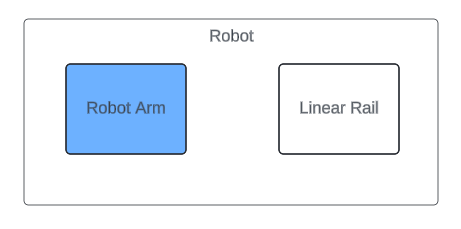
\includegraphics[width=0.60\textwidth]{images/Robot_Arm_Output.png}
 \caption{Robot Subsystem}
\end{figure}

\subsubsection{Subsystem Hardware}
The robot arm is a Mitsubishi RV-8CRL robot with an 8 kilogram payload.

\subsubsection{Subsystem Operating System}
N/A

\subsubsection{Subsystem Software Dependencies}
RT Toolbox.

\subsubsection{Subsystem Programming Languages}
MELFA BASIC VI.

\subsubsection{Subsystem Data Structures}
N/A.

\subsubsection{Subsystem Data Processing}
Signals from controller to robot arm to perform the movement, as well as signals from the PLC.

\subsection{Linear Rail}
Linear rail is being used as an additional axis to provide the robot a movement along an axis. It is considered to be the 7th axis of the robot in this case.

\begin{figure}[h!]
	\centering
 	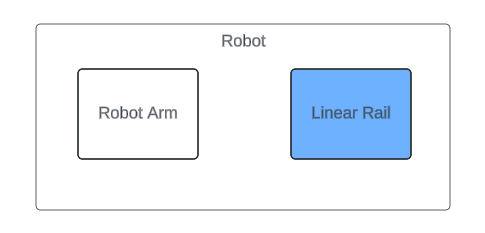
\includegraphics[width=0.60\textwidth]{images/linear_rail_output.png}
 \caption{Robot Subsystem}
\end{figure}

\subsubsection{Subsystem Hardware}
Linear rail itself.

\subsubsection{Subsystem Operating System}
N/A.

\subsubsection{Subsystem Software Dependencies}
RT Tool box.

\subsubsection{Subsystem Programming Languages}
MELFA BASIC VI.

\subsubsection{Subsystem Data Structures}
N/A.

\subsubsection{Subsystem Data Processing}
Signals from controller to robot arm to perform the movement.


\subsection{Air Compressor}
An air compressor is a pneumatic device that converts power (using an electric motor, diesel, or gasoline engine) into potential energy stored in pressurized air (also known as compressed air).

\begin{figure}[h!]
	\centering
 	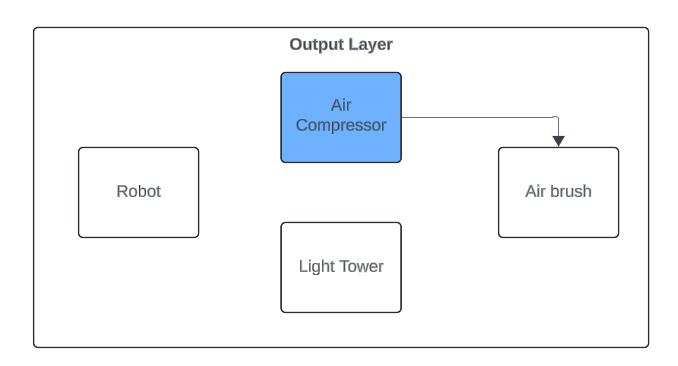
\includegraphics[width=0.60\textwidth]{images/AirCompressor_ouput.png}
 \caption{Air Compressor Subsystem}
\end{figure}

\subsubsection{Subsystem Hardware}
Air Compressor, as well as a solenoid switch triggered by PLC relay. Upon contact, air can flow through the pneumatic line to the robot and air brush.

\subsubsection{Subsystem Operating System}
N/A.

\subsubsection{Subsystem Software Dependencies}
GX Works.

\subsubsection{Subsystem Programming Languages}
Ladder diagram/logic.

\subsubsection{Subsystem Data Structures}
N/A.

\subsubsection{Subsystem Data Processing}
Signals from PLC to Air Compressor when to release pressure.

\subsection{Light Tower}
A light tower is a piece of mobile equipment that combines high-intensity electric lamps with a mast.

\begin{figure}[h!]
	\centering
 	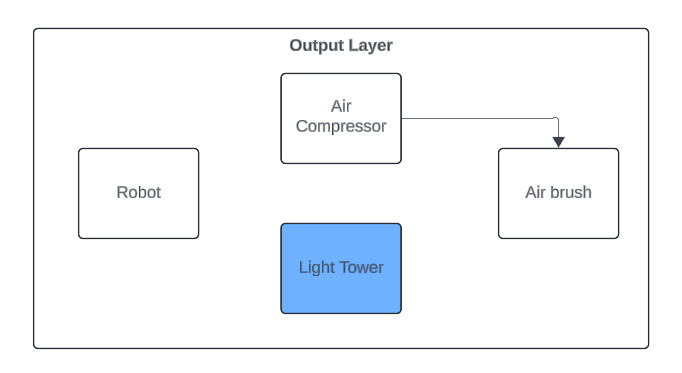
\includegraphics[width=0.60\textwidth]{images/LightTower_output.png}
 \caption{Pneumatic Control Subsystem}
\end{figure}

\subsubsection{Subsystem Hardware}
Light tower.

\subsubsection{Subsystem Operating System}
**Windows.

\subsubsection{Subsystem Software Dependencies}
GX Works.

\subsubsection{Subsystem Programming Languages}
Ladder Design/Logic.

\subsubsection{Subsystem Data Structures}
N/A.

\subsubsection{Subsystem Data Processing}
Signals flow from PLC to light tower indicating the status of robot.

\subsection{Air Brush}
An airbrush is a small, air-operated tool that atomizes and sprays various media, most often paint, but also ink, dye, and foundation.

\begin{figure}[h!]
	\centering
 	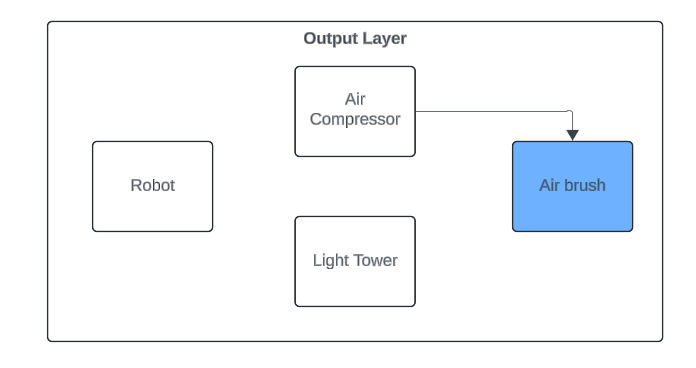
\includegraphics[width=0.60\textwidth]{images/AirBrush_output.png}
 \caption{Pneumatic Control Subsystem}
\end{figure}

\subsubsection{Subsystem Hardware}
**Air brush.

\subsubsection{Subsystem Operating System}
N/A.

\subsubsection{Subsystem Software Dependencies}
N/A.

\subsubsection{Subsystem Programming Languages}
N/A.

\subsubsection{Subsystem Data Structures}
N/A.

\subsubsection{Subsystem Data Processing}
There is no data which is being processed. Although air compressor sends air pressure when it is triggered by the PLC. The air pressure is passed through pneumatic lines.